\documentclass[user_manual.tex]{subfiles}
\begin{document}

%Inicio de la introducción
\chapter{Introducción}

El presente manual de usuario tiene como propósito ser una guía clara y específica para garantizar el uso y funcionamiento óptimo de Justina ``el robot de servicio'', resolver las dudas más comunes sobre el robot, así como la posibilidad de desarrollo de una replica del robot para su investigación. Comprende de la descripción general de los subsistemas de Justina.\\
\\
Se contempla todo lo relacionado al hardware empleado y se proveé de ligas para ver especificaciones más avanzadas, estas son dadas para el lector interesado en una explicación más detallada.\\
\\
Este documento contiene los algoritmos creados por los desarrolladores del laboratorio. Para cada modulo está incluida una breve descripción del algoritmo, técnicas o enfoques usados para el diseño.\\
\\
Cabe señalar, que, este documento esta sujeto a actualizaciones conforme sean requeridas por modificaciones hechas en el robot justina Justina.\\
\\
El robot de servicio Justina fue diseñado en el laboratorio Biorobotics, de la facultad de ingeniería de la UNAM.\\
\\
En la figura \ref{fig:introduction:Justina} se muestra el robot de servicio Justina.

%Figura 1.1 de Justina
\begin{figure}[H]
\centering
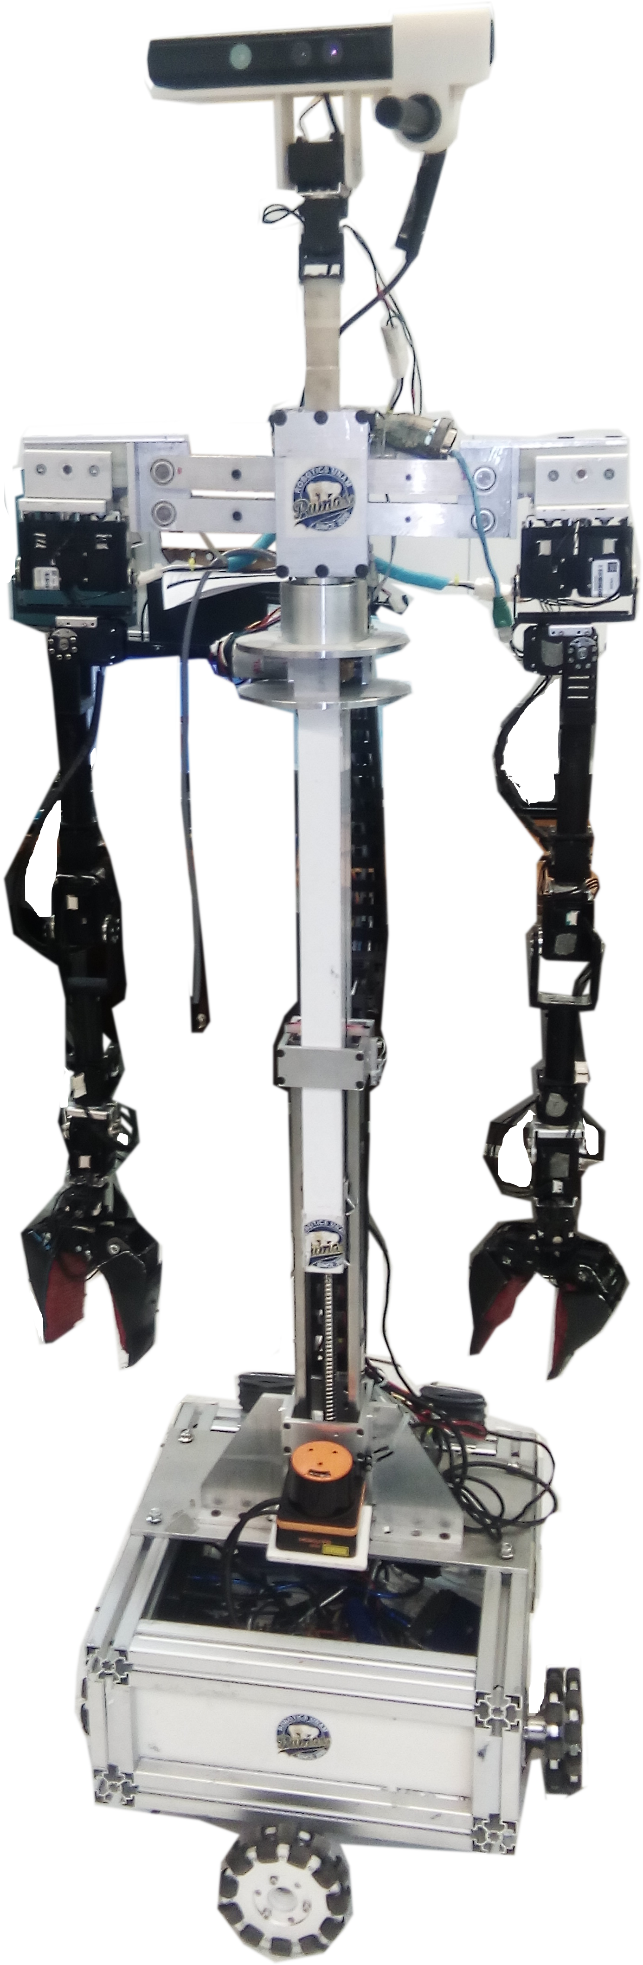
\includegraphics[width=0.7\textwidth]{Figures/Introduction/Justina.png}
\caption{El Robot Justina}
\label{fig:introduction:Justina}
\end{figure}
\pagebreak


\end{document}